\section{Exchange Metaheuristics}
\subsection{Overcoming local optima}
The steepest descent exchange heuristics only provide local optima.\\

In order to \textbf{improve}, one can
\begin{itemize}
	\item \textbf{repeat} the search (How to avoid following the same path?)
	\item \textbf{extend} the search (How to avoid falling in the same optimum? If I start in a neighborhood of my local optimum chances are I'll fall back into it)
\end{itemize}

In the constructive algorithms only repetition was possible.\\

The constructive metaheuristics exploit \textbf{randomization} and \textbf{memory} to operate on $\Delta_A^+ (x)$ and $\varphi_A (i, x)$.\\

The \textbf{exchange metaheuristics} exploit them to operate on
\begin{itemize}
	\item the \textbf{starting solution} $x^{(0)}$ (multi-start, ILS, VNS)
	\item the \textbf{neighborhood} $N (x)$ (VND)
	\item the \textbf{selection criteria} $\varphi (x, A, D)$ (DLS/GLS)
	\item the \textbf{selection rule} $\arg \min$ (SA, TS)
\end{itemize}

\newpage

\subsubsection{Termination condition} 

A search that repeats or extends beyond a local optimum can ideally be infinite. If you prolong the search, when does it end? \\

In practice, one uses \textbf{termination conditions} that can be "\textbf{absolute}"
\begin{enumerate}
	\item A given \textbf{total number of explorations of the neighborhood} or a given \textbf{total number of repetitions of the local search}.\\
	
	\item A given \textbf{total execution time}.\\
	
	\item A given \textbf{value of the objective}.\\
\end{enumerate}

or "\textbf{relative}" to the \textbf{profile of} $f^\ast$
\begin{enumerate}
	\item A given \textbf{number of explorations} of the neighborhood or repetitions \textbf{after the last improvement of} $f^\ast$.\\
	
	\item A given \textbf{execution time after the last improvement}.\\
	
	\item A given \textbf{minimum value of the ratio between improvement} of the objective and \textbf{number of explorations/repetitions} or \textbf{execution time} (e.g., $f^\ast$ improves less than $1\%$ in the last $1000$ explorations).\\
\end{enumerate}

\textbf{Fair comparisons} require \textbf{absolute conditions} (give both the same time/number of exploration).\\

\newpage

\subsection{Modify the starting solution}

It is possible to create \textbf{different starting solutions}
\begin{itemize}
	\item Generating them at \textbf{random}
	\begin{itemize}
		\item with uniform probability
		\item with biased distributions (based on the data, possibly on memory)
	\end{itemize}
	\nn
	
	\item Applying different \textbf{constructive algorithms}
	\begin{itemize}
		\item heuristics
		\item metaheuristics (with randomization and/or memory)
	\end{itemize}
	\nn
	
	\item Applying the \textbf{exchange algorithm to modify the solutions visited} (therefore with memory, and usually also randomization)
\end{itemize}

\newpage

\subsubsection{Random generation}

The \textbf{advantages} of random generation are
\begin{itemize}
	\item Conceptual \textbf{simplicity}.\\
	
	\item \textbf{Quickness} for the problems in which it is easy to guarantee feasibility.\\
	
	\item \textbf{Control} on the \textbf{probability distribution} in $X$ based on
	\begin{itemize}
		\item element cost (e.g., favor the cheapest elements)
		
		\item element frequency during the past search, to favor the most frequent elements (intensification) or the less frequent ones (diversification). This combines randomization and memory
	\end{itemize}
	\nn
	
	\item \textbf{Asymptotic convergence to the optimum} (in infinite time).\\
\end{itemize}


The \textbf{disadvantages} of random generation are
\begin{itemize}
	\item \textbf{Scarce quality} of the \textbf{starting solutions} (not the final ones).\\
	
	\item \textbf{Long times} before \textbf{reaching the local optimum}. This depends on the complexity of the exchange algorithm.\\
	
	\item \textbf{Inefficiency} when deciding feasibility is $\mathcal{NP}$-complete.\\
\end{itemize}

\newpage

\subsubsection{Constructive procedures}

Multi-start methods are the classical approach
\begin{itemize}
	\item design \textbf{several constructive heuristics}
	\item \textbf{each} constructive heuristic \textbf{generates a starting solution}
	\item \textbf{each starting solution} is \textbf{improved} by the \textbf{exchange heuristic}
\end{itemize}

\nn

The disadvantages are
\begin{enumerate}
	\item \textbf{scarce control}: the generated solutions tend to be similar
	
	\item \textbf{impossibility to proceed indefinitely}: the number of repetitions is fixed
	
	\item \textbf{high design effort}: several different algorithms must be designed
	
	\item \textbf{no guarantee of convergence}, not even in infinite time
\end{enumerate}

Consequently, constructive metaheuristics are preferred nowadays. The initial step is given by a constructive metaheuristic. \\

GRASP and Ant System include by definition an exchange procedure.\\

What's the difference between a metaheuristic with a randomized/memory based constructive phase and an exchange heuristic with initialized by a randomized process? There's little difference.\\

\newpage

\subsubsection{Influence of the starting solution}
The starting solution obviously has influence on the algorithm's performance, so how do we determine if we can choose a random generation or if we need a good constructive heuristic?\\

If the \textbf{exchange heuristic} is
\begin{itemize}
	\item \textbf{Good}, the starting solution has a \textbf{short-lived influence}: a random or heuristic generation of $x^{(0)}$ are very similar.\\
	
	\item \textbf{Bad}, the starting solution has a \textbf{long-lived influence}: a good heuristic to generate $x^{(0)}$ is useful.\\
\end{itemize}
If the heuristic is not good, it might be a good idea to spend some time generating the starting solution, while if the exchange phase is very good the starting solution doesn't matter as much.\\

\begin{center}
	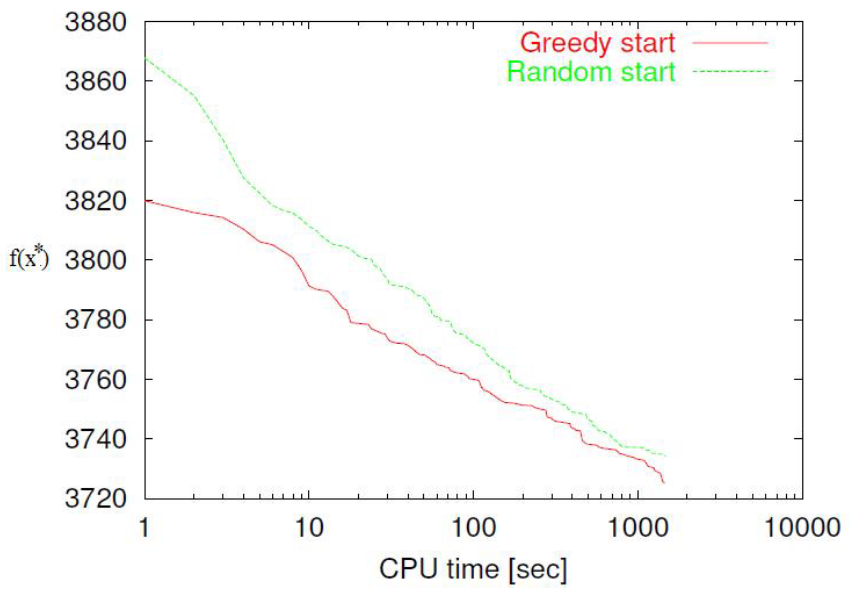
\includegraphics[width=0.8\columnwidth]{img/influence1}
\end{center}
\textit{This exchange heuristic is not very good, there's still a perceivable (albeit small) difference at the end, after a significant amount of time (note the logarithmic scale).}

\newpage

\subsubsection{Exploiting the previous solutions}
The idea is to \textbf{exploit the information on previously visited solutions}
\begin{itemize}
	\item save \textbf{reference solutions}, such as the best local optimum found so far and possibly other local optima
	
	\item \textbf{generate the new starting solution modifying the reference ones}
\end{itemize}

During the exchange heuristic you save some solutions that are "interesting" (the best, possibly others, usually good-quality solutions) and generate some other starting solutions based on these.\\ 

The advantages of this approach are
\begin{itemize}
	\item \textbf{control}: the modification can be reduced or increased \textit{ad libitum}. You can intensify or diversify the search at will (in respect to the starting point)
	
	\item \textbf{good quality}: the starting solution is very good (you start from a good-quality solution)
	
	\item \textbf{conceptual simplicity}: just design a modification, no need to invent much new stuff
	
	\item \textbf{implementation simplicity}: the modification can be performed with the operations defining the neighborhood
	
	\item \textbf{asymptotic convergence to the optimum} under suitable conditions
\end{itemize}

\newpage

\subsection{Iterated Local Search (ILS)}

The Iterated Local Search (ILS), proposed by Louren¸co, Martin and St\"utzle (2003) requires
\begin{itemize}
	\item a \textbf{steepest descent} exchange heuristic to \textbf{produce local optima}
	
	\item a \textbf{perturbation procedure} to \textbf{generate the starting solutions}
	
	\item an \textbf{acceptance condition} to decide whether to \textbf{change the reference solution} $x$
	
	\item a \textbf{termination condition}
\end{itemize}

\begin{algorithm}
	\caption{Algorithm $IteratedLocalSearch(I , x^{(0)})$}
	\begin{algorithmic}
		\STATE $x := SteepestDescent(x^{(0)})$
		\STATE $x^\ast := x$
		\FOR{$l := 1$ to $\ell$}
		\STATE $x' := Perturbate(x)$
		\STATE $x' := SteepestDescent(x')$
		\IF{$Accept(x', x^\ast)$} 
		\STATE $x := x'$
		\ENDIF
		\IF{$f (x') < f (x^\ast)$}
		\STATE $x^\ast := x'$
		\ENDIF
		\ENDFOR
		\RETURN $(x^\ast, f (x^\ast))$
	\end{algorithmic}
\end{algorithm}

It iteratively applies local search by generating new starting solutions every time, so you need an exchange heuristic on which to base this on.\\

The perturbation procedure is used to generate new starting solutions from the reference.\\

The acceptance condition is needed to decide if the local optimum found can be accepted as the new reference (otherwise the old one is kept and "perturbed" for a new starting solution).\\

In the end it returns the best solution found.

\newpage

The idea is that
\begin{itemize}
	\item The \textbf{exchange heuristic quickly explores an attraction basin}, terminating into a local optimum.
	
	\item The \textbf{perturbation procedure moves to another attraction basin}.
	
	\item The \textbf{acceptance condition evaluates if the new local optimum is a promising starting point} for the following perturbation.
\end{itemize}

\begin{center}
	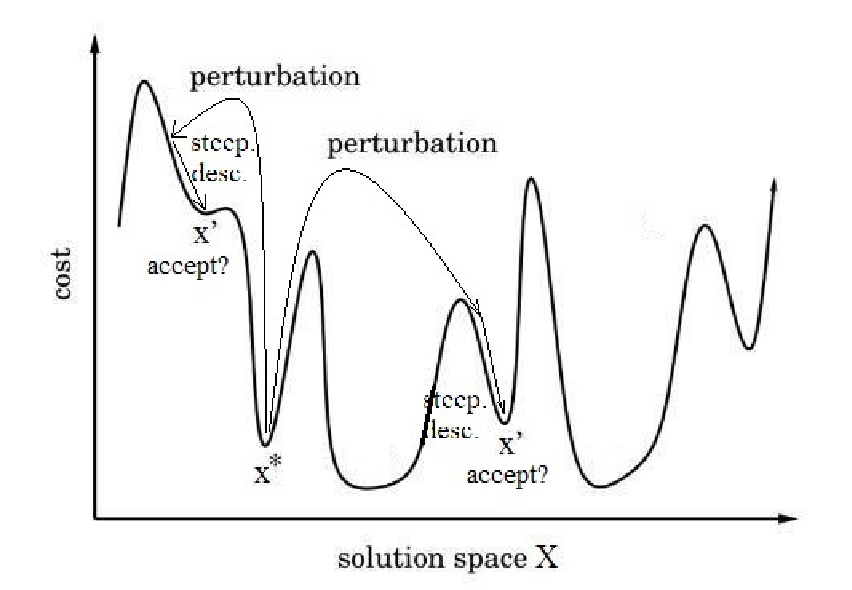
\includegraphics[width=0.7\columnwidth]{img/ILS1}
\end{center}

\vfill

\paragraph{Example:} A classical application of ILS to the TSP uses
\begin{itemize}
	\item exchange heuristic: steepest descent with neighborhood $N_{\mathcal{R}_2}$ (remove 2 edges)
	
	\item perturbation procedure: a double-bridge move that is particular kind of 4-exchange
	\begin{center}
		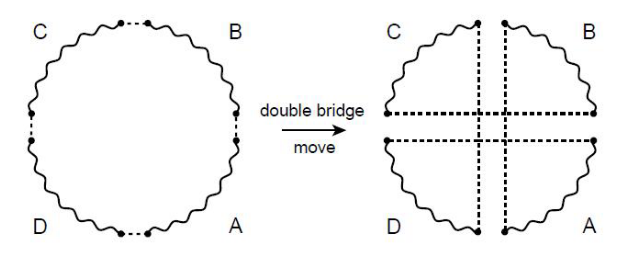
\includegraphics[width=0.6\columnwidth]{img/TSP5}
	\end{center}
	
	\item acceptance condition: the best known solution improves 
	$$f (x') < f (x^\ast)$$
	The reference solution is the best known one ($x = x^\ast$)
\end{itemize}

\newpage

\subsubsection{Perturbation procedure}

Let $\mathcal{O}$ be the operation set that defines neighborhood $N_{\mathcal{O}}$.\\

The \textbf{perturbation procedure} performs a \textbf{random operation} $o$
\begin{itemize}
	\item with $o \in \mathcal{O}' \not \subseteq \mathcal{O}$, to avoid the exchange heuristic driving solution $x'$ back to the starting local optimum $x$ (you need a new starting point, go far enough to get one)
\end{itemize}

Two typical definitions of $\mathcal{O}'$ are
\begin{itemize}
	\item \textbf{sequences of} $k > 1$ \textbf{operations of} $\mathcal{O}$ (generating a random sequence is cheap)
	
	\item \textbf{conceptually different operations} (e.g., vertex exchanges instead of edge exchanges)
\end{itemize}

The main difficulty of ILS is in tuning the perturbation: if it is
\begin{itemize}
	\item \textbf{Too strong}, it turns the search into a \textbf{random restart} (if you go way too far it's just a new random start).\\
	
	\item \textbf{Too weak}, it guides the search back to the \textbf{starting local optimum} (you are too close to the previous one)
	\begin{itemize}
		\item wasting time
		\item possibly losing the asymptotic convergence
	\end{itemize}
	\nn
\end{itemize}

Ideally one would like to \textbf{enter any basin} and \textbf{get out of any basin} (and the perturbation must be tuned according to the specific basin).\\

\newpage

\subsubsection{Acceptance condition}
The acceptance condition \textbf{balances intensification and diversification}
\begin{itemize}
	\item Accepting \textbf{only improving solutions} favors \textbf{intensification}
	$$Accept(x', x^\ast) := (f (x') < f (x^\ast))$$
	The reference solution is always the best found: $x = x^\ast$.\\
	
	\item Accepting \textbf{any solution} favors \textbf{diversification}
	$$ Accept(x', x^\ast) := true $$
	The reference solution is always the last optimum found: $x = x'$.\\
\end{itemize}

\textbf{Intermediate strategies} can be defined \textbf{based on} $\delta f = f (x') - f (x^\ast)$ the difference in the objective function
\begin{itemize}
	\item if $\delta f < 0$, \textbf{always accept} $x'$
	
	\item if $\delta f \geq 0$, \textbf{accept} $x'$ \textbf{with probability} $\pi (\delta f)$, where $\pi (\cdot)$ is a nonincreasing function
\end{itemize}

The most \textbf{typical cases} are:
\begin{itemize}
	\item \textbf{constant probability}: $\pi (\delta f ) = \overline{\pi} \in (0; 1)$ for each $\delta f \geq 0$
	
	\item \textbf{monotonically decreasing probability} with $\pi (0) = 1$ and $\lim_{\delta f \rightarrow + \infty} \pi (\delta) = 0$; the probability decreases proportionally to the worsening of the solution
\end{itemize}

\begin{center}
	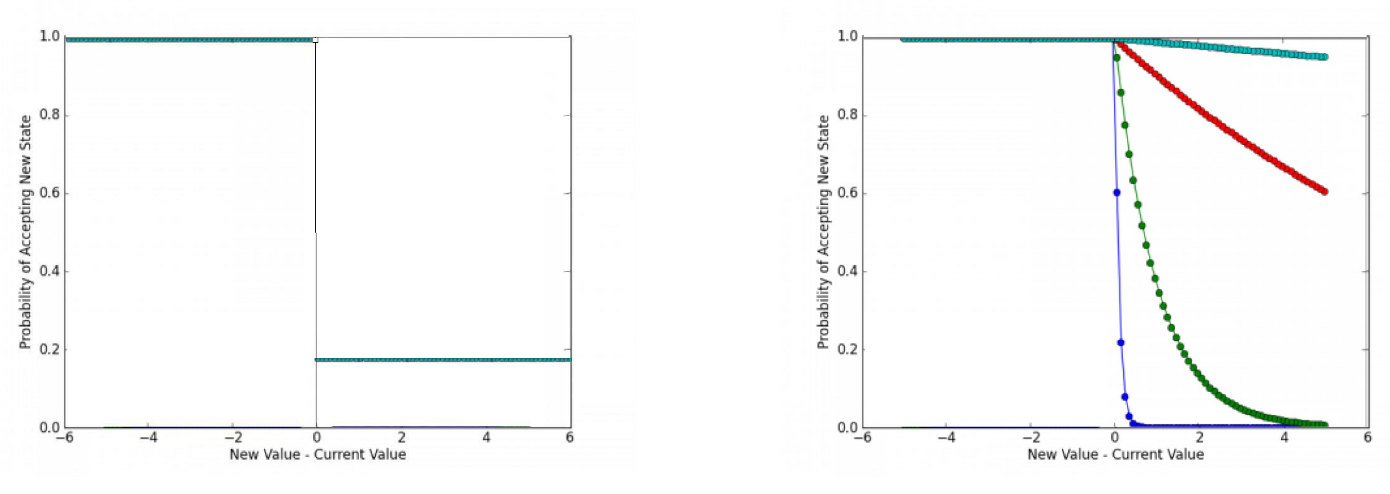
\includegraphics[width=\columnwidth]{img/accept1}
\end{center}

\textbf{Memory} can also be used, \textbf{accepting} $x'$ \textbf{more easily if many iterations have elapsed since the last improvement of} $x^\ast$.\\

\newpage

\subsection{Variable Neighborhood Search (VNS)}

A method very similar to ILS is the Variable Neighborhood Search proposed by Hansen and Mladenovi\'c (1997).\\

The \textbf{main differences} between ILS and VNS are the \textbf{use of}
\begin{itemize}
	\item The \textbf{strict acceptance condition}: $f (x') < f (x^\ast)$ (only intensifies, simpler).\\
	
	\item An \textbf{adaptive perturbation mechanism} instead of the fixed one (more complicated than ILS).\\
\end{itemize}

VNS often introduces also neighborhood modifications (later on this).\\

The \textbf{perturbation mechanism} is based on a \textbf{hierarchy of neighborhoods}, that is a \textbf{family of neighborhoods with an increasing parametric size} $s$
$$ N_1 \subset N_2 \subset \, ... \, \subset N_s \subset \, ... \, N_{s_{max}} $$


Typically, the parameterized neighborhoods used are
\begin{itemize}
	\item $N_{\mathcal{H}_s}$, based on the Hamming distance between subsets
	
	\item $N_{\mathcal{O}_s}$, based on the sequences of operations from a basic set $\mathcal{O}$
\end{itemize}

and $x^{(0)}$ is extracted randomly from a neighborhood of the hierarchy.\\

\newpage

\begin{algorithm}
	\caption{Algorithm $VariableNeighbourhoodSearch(I , x^{(0)}, s_{min}, s_{max}, \delta s)$}
	\begin{algorithmic}
		\STATE $x := SteepestDescent(x^{(0)})$ 
		\STATE $x^\ast := x$
		\STATE $s := s_{min}$
		\FOR{$l := 1$ to $\ell$}
		\STATE $x' := Shaking(x^\ast, s)$
		\STATE $x' := SteepestDescent(x')$
		\IF{$f (x') < f (x^\ast)$}
		\STATE $x^\ast := x'$
		\STATE $s := s_{min}$
		\ELSE 
		\STATE $s := s + \delta s$
		\ENDIF
		\IF{$s > s_{max}$}
		\STATE $s := s_{min}$
		\ENDIF
		\ENDFOR
		\RETURN $(x^\ast, f (x^\ast))$
	\end{algorithmic}
\end{algorithm}

\begin{itemize}
	\item the \textbf{reference solution} $x'$ is \textbf{always the best known} solution $x^\ast$
	
	\item the \textbf{starting solution} is obtained extracting it at \textbf{random from the current neighborhood of the reference solution} $N_s (x^\ast)$
	
	\item the \textbf{exchange heuristic} produces a \textbf{local optimum} with respect to the \textbf{basic neighborhood} $N$
	
	\item if the \textbf{best known solution improves}, the \textbf{current neighborhood becomes} $N_{s_{min}}$
	
	\item \textbf{otherwise, move to a larger neighborhood} $N_{s+\delta s}$, never exceeding $N_{s_{max}}$
\end{itemize}

\newpage

\subsubsection{Adaptive perturbation mechanism}
It is called \textbf{variable neighborhood} because the \textbf{neighborhood used to extract} $x^{(0)}$ \textbf{varies} based on the results of the exchange heuristic
\begin{itemize}
	\item \textbf{if a better solution is found}, use the \textbf{smallest neighborhood}, to generate a starting solution very close to $x^\ast$ (intensification)
	
	\item \textbf{if a worse solution is found}, use a \textbf{slightly larger neighborhood}, to generate a starting solution slightly farther from $x^\ast$ (diversification)
\end{itemize}

If you find a better solution you accept it and set $s$ to the minimum possible value, the new starting solution is close to the current one (you get closer, perturb only a little).\\
If you find a worse solution you perturbed too little, you need to increase $s$ and perturb more (starting solution that is farther away from the current one).\\


The method has \textbf{three parameters}
\begin{enumerate}
	\item $s_{min}$ identifies the \textbf{smallest neighborhood to generate new solutions}
	
	\item $s_{max}$ identifies the \textbf{largest neighborhood to generate new solutions}
	
	\item $\delta_s$ is the \textbf{increase of} $s$ \textbf{between two subsequent attempts} (how much does the neighborhood increase when it fails?)
\end{enumerate}

The exchange heuristic adopts a \textbf{small neighborhood to be efficient} ($N_1$, or anyway $N_s$ with $s \leq s_{min}$).\\

\newpage

\paragraph{Tuning of the shaking parameters:} The value of $s_{min}$ must be
\begin{itemize}
	\item \textbf{Large enough} to get \textbf{out of the current attraction basin}.\\
	
	\item \textbf{Small enough} to \textbf{avoid jumping over the adjacent attraction basins}.\\
\end{itemize}

In general, one sets $s_{min} = 1$, and increases it if experimentally profitable.\\

The value of $s_{max}$ must be
\begin{itemize}
	\item \textbf{Large enough} to \textbf{reach any useful attraction basin}.\\
	
	\item \textbf{Small enough} to \textbf{avoid reaching useless regions} of the solution space.\\
\end{itemize}
Example: the diameter of the search space for the basic neighborhood: $\min (k, n - k)$ for the MDP; $n$ for the TSP and MAX-SAT, etc.\\

The value of $\delta s$ must be
\begin{itemize}
	\item \textbf{Large enough} to \textbf{reach} $s_{max}$ \textbf{in a reasonable time}.\\
	
	\item \textbf{Small enough} to \textbf{allow each reasonable value of} $s$.\\
\end{itemize}

In general, one sets $\delta s = 1$, unless $s_{max} - s_{min}$ is too large.\\

\newpage

\subsubsection{Skewed VNS}
In order to \textbf{favor diversification}, it is possible to \textbf{accept} $x'$ \textbf{when}
$$ f (x') < f (x^\ast) + \alpha d_{\mathcal{H}} (x', x^\ast) $$
where
\begin{itemize}
	\item $d_{\mathcal{H}} (x', x^\ast)$ is the \textbf{Hamming distance} between $x'$ and $x^\ast$
	
	\item $\alpha > 0$ is a \textbf{suitable parameter}
\end{itemize}
Accept bounded worsening solution, if they're far enough away (measured with the Hamming distance). How distant they are determines how much worse they can get.\\

This allows to \textbf{accept worsening solutions} as long as they are \textbf{far away}
\begin{itemize}
	\item $\alpha \approx 0$ tends to accept only improving solutions
	
	\item $\alpha \gg 0$ tends to accept any solution
\end{itemize}
The parameter $\alpha$ is the "worsening bound", determines how much worse the solution can get and still get accepted (if it's far enough away).\\

Of course, the random strategies seen for the ILS can also be adopted.\\

% End of L17

\newpage

\subsection{Extending the local search without worsening}

Instead of repeating the local search, \textbf{extend it beyond the local optimum}.\\

To \textbf{avoid worsening} solutions, the \textbf{selection step must be modified}
$$ \tilde{x} := \arg \min_{x' \in N(x)} f (x') $$

And two main strategies allow doing that
\begin{itemize}
	\item The \textbf{Variable Neighborhood Descent} (VND), \textbf{changes the neighborhood} $N$
	\begin{itemize}
		\item it guarantees an evolution with no cycles (the objective improves)
		\item it terminates when all neighborhoods have been exploited
	\end{itemize}
	\nn
	
	\item The \textbf{Dynamic Local Search} (DLS) \textbf{changes the objective function} $f$ ($\tilde{x}$ is better than $x$ for the new objective, possibly worse for the old)
	\begin{itemize}
		\item it can be trapped in loops (the new objective changes over time)
		\item it can proceed indefinitely
	\end{itemize}
	\nn
\end{itemize}

\newpage

\subsection{Variable Neighborhood Descent (VND)}

The Variable Neighborhood Descent of Hansen and Mladenovi\'c (1997) exploits the fact that a \textbf{solution is locally optimal for a specific neighborhood}
\begin{itemize}
	\item a \textbf{local optimum} can be \textbf{improved} using a \textbf{different neighborhood}
\end{itemize}
If you change the neighborhood, the local optimum changes.\\

Given a \textbf{family of neighborhoods} $N_1, \, ... \, , N_{s_{tot}}$
\begin{enumerate}
	\item set $s := 1$
	\item apply a \textbf{steepest descent exchange heuristic} and find a \textbf{local optimum} $\overline{x}$ \textbf{with respect to} $N_s$
	\item \textbf{flag all neighborhoods} for which $\overline{x}$ \textbf{is locally optimal and update} $s$
	\item if $\overline{x}$ is a local optimum for all $N_s$, terminate; otherwise, go back to point 2
\end{enumerate}

\begin{algorithm}
	\caption{Algorithm $VariableNeighbourhoodDescent(I , x^{(0)})$}
	\begin{algorithmic}
		\STATE $flag_s := false \; \forall k$
		\STATE $\overline{x} := x^{(0)}$ 
		\STATE $x^\ast := x^{(0)}$
		\STATE $s := 1$
		\WHILE{$\exists s : flag_s = false$}
		\STATE $\overline{x} := SteepestDescent(\overline{x}, s)$ // possibly truncated
		\STATE $flag_s := true$
		\IF{$f (\overline{x}) < f (x^\ast)$}
		\STATE $x^\ast := \overline{x}$
		\STATE $flag_{s'} := false \; \forall s' \neq s$
		\ENDIF
		\STATE $s := Update(s)$
		\ENDWHILE
		\RETURN $(x^\ast, f (x^\ast))$
	\end{algorithmic}
\end{algorithm}

\newpage

\paragraph{Anticipated termination of Steepest Descent:} Using many neighborhoods means that some might be rather \textbf{large} and \textbf{slow to explore}.\\

In order to increase the efficiency of the method one can
\begin{itemize}
	\item Adopt a \textbf{first-best strategy in the larger neighborhoods}.\\
	
	\item \textbf{Terminate the Steepest Descent before reaching a local optimum} (possibly even after a single step).\\
	
\end{itemize}
Larger neighborhoods aim to \textbf{move out of the basins of attraction of smaller ones}.\\

\nn

\paragraph{VND and VNS:} There is of course a strict relation between VND and VNS (in fact, they were proposed in the same paper).\\

The \textbf{fundamental differences} are that in the VND
\begin{itemize}
	\item At each step the \textbf{current solution is the best known one}.\\
	
	\item The \textbf{neighborhoods are explored}, instead of being used to extract random solutions; they are never huge.\\
	
	\item The \textbf{neighborhoods do not necessarily form a hierarchy}; the update of $s$ is not always an increment.\\
	
	\item When a \textbf{local optimum for each} $N_s$ \textbf{has been reached}, \textbf{terminate}; VND is deterministic and would not find anything else.\\
\end{itemize}

\newpage

\subsubsection{Neighborhood update strategies for the VND}

There are two main classes of VND methods:
\begin{itemize}
	\item with \textbf{heterogeneous neighborhoods}
	\begin{itemize}
		\item exploit the potential of \textbf{topologically different neighborhoods} (e.g., exchange vertices instead of edges)
	\end{itemize}
	Consequently, $s$ periodically scans the values from $1$ to $s_{tot}$ (possibly randomly permuting the sequence at each repetition).\\
	
	\item with \textbf{hierarchical neighborhoods} ($N_1 \subset \, ... \, \subset N_{s_{tot}}$)
	\begin{itemize}
		\item \textbf{fully exploit} the \textbf{small and fast neighborhoods}
		\item resort to the \textbf{large and slow ones only to get out of local optima} (usually terminating Steepest Descent prematurely)
	\end{itemize}
	Consequently, the update of $s$ works as in the VNS
	\begin{itemize}
		\item when \textbf{no improvements} can be found in $N_s$, \textbf{increase} $s$
		\item when \textbf{improvements} can be found in $N_s$, \textbf{decrease} $s$ back to $1$
	\end{itemize}
\end{itemize}

\textbf{Terminate when the current solution is a local optimum for all} $N_s$
\begin{itemize}
	\item in the \textbf{heterogeneous case}, terminate when \textbf{all fail}
	\item in the \textbf{hierarchical case}, terminate when the \textbf{largest fails}
\end{itemize}

\newpage

\paragraph{Example:} This instance of CMSTP has $n = 9$ vertices, uniform weights ($w_v = 1$), capacity $W = 5$ and the reported costs (graph is complete, but the missing edges have $c_e \gg 3$, so they are not drawn).

\begin{center}
	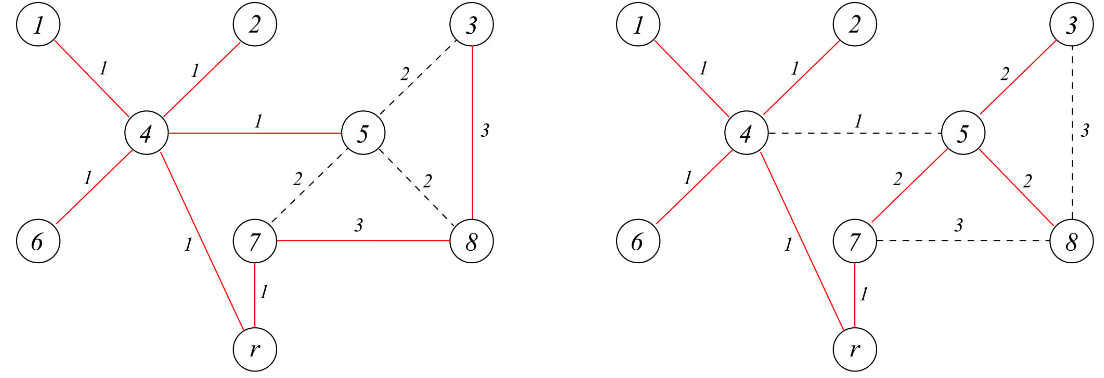
\includegraphics[width=\columnwidth]{img/CMST4}
\end{center}

Consider neighborhood $N_{\mathcal{S}_1}$ (single-edge swaps) for the first solution:
\begin{itemize}
	\item no edge in the right branch can be deleted because the left branch has zero residual capacity and a direct connection to the root would increase the cost
	
	\item deleting any edge in the left branch increases the total cost, the solution is a local optimum for $N_{\mathcal{S}_1}$
\end{itemize} 

Neighborhood $N_{\mathcal{T}_1}$ (single-vertex transfers) has an improving solution, obtained moving vertex $5$ from the left branch to the right one.\\

On the left the solution for $N_{\mathcal{S}_1}$, on the right the one for $N_{\mathcal{T}_1}$ (obviously the case of heterogeneous neighborhoods).\\

\newpage

\subsection{Dynamic Local Search (DLS)}

The Dynamic Local Search is also known as Guided Local Search.\\

Its approach is \textbf{complementary} to VND
\begin{itemize}
	\item it \textbf{keeps the starting neighborhood}
	\item it \textbf{modifies the objective function}
\end{itemize}

It is often used when the \textbf{objective is useless} because it has \textbf{wide plateaus} (e.g. in the PMSP the completion time is often the same, even after multiple movements).\\

The \textbf{basic idea} is to
\begin{itemize}
	\item Define a \textbf{penalty function} $w : X \rightarrow \mathbb{N}$ (defined on the solution, usually integer values).\\
	
	\item Build an \textbf{auxiliary function} $\tilde{f} (f (x) , w (x))$ which \textbf{combines the objective function} $f$ \textbf{with the penalty} $w$.\\
	
	\item Apply a \textbf{steepest descent exchange heuristic to optimize} $\tilde{f}$.\\
	
	\item At each iteration \textbf{update the penalty} $w$ \textbf{based on the results} (and consequently update the function $\tilde{f}$ and the landscape of the search).\\
\end{itemize}

The penalty is adaptive in order to move away from recent local optima, but this introduces the risk of cycling.\\

\newpage

\begin{algorithm}
	\caption{Algorithm $DynamicLocalSearch(I , x^{(0)})$}
	\begin{algorithmic}
		\STATE $w := StartingPenalty(I )$
		\STATE $\overline{x} := x^{(0)}$
		\STATE $x^\ast := x^{(0)}$
		\WHILE{$Stop() = false$}
		\STATE $(\overline{x}, x_f) := SteepestDescent(\overline{x}, f , w )$ // possibly truncated
		\IF{$f (x_f ) < f (x^\ast)$}
		\STATE $x^\ast := x_f$
		\ENDIF
		\STATE $w := UpdatePenalty(w, \overline{x}, x^\ast)$
		\ENDWHILE
		\RETURN $(x^\ast, f (x^\ast))$
	\end{algorithmic}
\end{algorithm}
Notice that the steepest descent heuristic
\begin{itemize}
	\item \textbf{Optimizes a combination} $\tilde{f}$ \textbf{of} $f$ \textbf{and} $w$ (Steepest Descent is applied to both).\\
	
	\item \textbf{Returns two solutions}:
	\begin{enumerate}
		\item a \textbf{final solution} $\overline{x}$, locally \textbf{optimal} with \textbf{respect to} $\tilde{f}$, \textbf{to update} $w$
		\item a \textbf{solution} $x_f$, that is the \textbf{best it has found with respect to} $f$
	\end{enumerate}
\end{itemize}

\newpage

\subsubsection{Variants}

The \textbf{penalty can be applied} (for example)
\begin{itemize}
	\item \textbf{Additively} to the elements of the solution:
	$$ \tilde{f} (x) = f (x) + \sum_{i \in x} w_i $$
	The function becomes the sum of the objective with the sum of the penalties for all elements in the solution; each element is penalized, it searches for elements with low penalty.\\
	
	\item \textbf{Multiplicatively} to components of the objective $f (x) = \sum_j \phi_j (x)$:
	$$ \tilde{f} (x) = \sum_j w_j \phi_j (x) $$
	The objective function is defined in terms of components and each one is multiplied by its penalty.\\
\end{itemize}

The \textbf{penalty} can be \textbf{updated}
\begin{itemize}
	\item at \textbf{each} single \textbf{neighborhood exploration}
	
	\item when a \textbf{local optimum for} $\tilde{f}$ \textbf{is reached}
	
	\item when the \textbf{best known solution} $x^\ast$ \textbf{is unchanged for a long time}
\end{itemize}
\nn

The \textbf{penalty} can be \textbf{modified} with
\begin{itemize}
	\item \textbf{Random updates}: "noisy" perturbation of the costs.\\
	
	\item \textbf{Memory-based updates}, favoring the most frequent elements (intensification) or the less frequent ones (diversification).\\
\end{itemize}

These two are not the only ways, they are just examples, more can be defined.\\

\newpage

\paragraph{Example:} DLS for the MCP. Given an undirected graph, find a maximum cardinality clique (subset of vertices that are fully connected)
\begin{itemize}
	\item The exchange heuristic is a VND using the neighborhoods
	\begin{enumerate}
		\item $N_{\mathcal{A}_1}$ (vertex addition): the solution always improves, but the neighborhood is very small and often empty
		
		\item $N_{\mathcal{S}_1}$ (exchange of an internal vertex with an external one): the neighborhood is larger, but forms a plateau (uniform objective)
	\end{enumerate}
	\nn
	
	\item The objective provides no useful direction in either neighborhood.\\
	
	\item Associate to each vertex $i$ a penalty $w_i$ initially equal to zero.\\
	
	\item The exchange heuristic minimizes the total penalty (within the neighborhood).\\
	
	\item Update the penalty
	\begin{enumerate}
		\item when the exploration of $N_{\mathcal{S}_1}$ terminates: the penalty of the current clique vertices increases by $1$
		
		\item after a given number of explorations: all the nonzero penalties decrease by 1
	\end{enumerate}
	\nn
\end{itemize}

The rationale of the method consists in aiming to
\begin{itemize}
	\item expel the internal vertices (diversification)
	\item in particular, the oldest internal vertices (memory)
\end{itemize}

\newpage

\begin{center}
	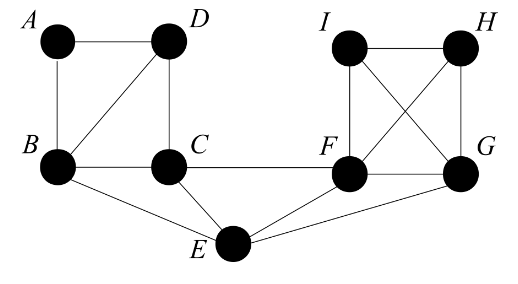
\includegraphics[width=0.6\columnwidth]{img/MCP2}
\end{center}

Start from $x^{(0)} = \{B, C , D\}$, with $w = [\; 0 \; 1 \; 1\; 1\; 0\; 0\; 0\; 0\; 0\; ]$
\begin{enumerate}
	\item $w (\{B, C , E \}) = w (\{A, B, D\}) = 2$, but $\{A, B, D\}$ wins lexicographically: $x^{(1)} = \{A, B, D\}$ with $w = [\; 1\; 2\; 1\; 2\; 0\; 0\; 0\; 0\; 0\; ]$
	
	\item $x^{(2)} = \{B, C , D\}$ with $w = [\; 1\; 3\; 2\; 3\; 0\; 0\; 0\; 0\; 0\; ]$ is the only neighbor
	
	\item $w (\{B, C , E \}) = 5 < 7 = w (\{A, B, D\})$: $x^{(3)} = \{B, C , E \}$ with $w = [\; 1\; 4\; 3\; 3\; 1\; 0\; 0\; 0\; 0\; ]$
	
	\item $w (\{C , E , F \}) = 4 < 10 = w (\{B, C , D\})$: $x^{(4)} = \{C , E , F \}$ with $w = [\; 1\; 4\; 4\; 3\; 2\; 1\; 0\; 0\; 0\; ]$
	
	\item $w (\{E , F , G \}) = 3 < 11 = w (\{B, C , E \})$: $x^{(5)} = \{E , F , G \}$ with $w = [\; 1\; 4\; 4\; 3\; 3\; 2\; 1\; 0\; 0\; ]$
	
	\item $w (\{F , G , H\}) = w (\{F , G , I \}) = 3 < 9 = w (\{C , E , F \})$: $x^{(6)} = \{F , G , H\}$ with $w = [\; 1\; 4\; 4\; 3\; 3\; 3\; 2\; 1\; 0\; ]$
\end{enumerate}

Now the neighborhood $N_{\mathcal{A}_1}$ is not empty: $x^{(7)} = \{F , G , H, I \}$

\newpage

\paragraph{Example:} DLS for the MAX-SAT. Given $m$ logical disjunctions depending on $n$ logical variables, find a truth assignment satisfying the maximum number of clauses
\begin{itemize}
	\item Neighborhood $N_{\mathcal{F}_1}$ (1-flip) is generated complementing a variable.\\
	
	\item Associate to each logical clause a penalty $w_j$ initially equal to $1$ (each component is a satisfied formula).\\
	
	\item The exchange heuristic maximizes the weight of satisfied clauses thus modifying their number with the multiplicative penalty.\\
	
	\item The penalty is updated
	\begin{enumerate}
		\item increasing the weight of unsatisfied clauses to favor them
		$$ w_j := \alpha_{us} w_j \text{ for each } j \in U (x) \; (\text{with } \alpha_{us} > 1) $$
		when a local optimum is reached
		
		\item reducing the penalty towards 1
		$$ w_j := (1 - \rho) w_j + \rho \cdot 1 \text{ for each } j \in C (\text{with } \rho \in (0, 1)) $$
		with a certain probability or after a certain number of updates
	\end{enumerate}
\end{itemize}

The rationale of the method consists in aiming to
\begin{itemize}
	\item satisfy the currently unsatisfied clauses (diversification)
	
	\item in particular, those which have been unsatisfied for longer time and more recently (memory)
\end{itemize}

The parameters tune intensification and diversification
\begin{itemize}
	\item small values of $\alpha_{us}$ and $\rho$ preserve the current penalty (intensification)
	
	\item large values of $\alpha_{us}$ push away from the current solution (diversification)
	
	\item large values of $\rho$ lead push towards the local optimum of the current attraction basin (a different kind of intensification)
\end{itemize}

% End of L18

\newpage

\subsection{Extending the local search with worsenings}

If the neighborhood and objective remain the same, the rule of acceptance must change: instead of
$$ x' := \arg \min_{x\in N(x)} f (x) $$
\textbf{select a nonminimal (possibly, even non-improving) solution}.\\

The main problem is the \textbf{risk of cyclically visiting the same solutions}.\\

The two main strategies that allow to control this risk are
\begin{itemize}
	\item \textbf{Simulated Annealing} (SA), which uses \textbf{randomization} to make repetitions unlikely.\\
	
	\item \textbf{Tabu Search} (TS), which uses \textbf{memory} to forbid repetitions.\\
\end{itemize}

\newpage

\subsection{Simulated Annealing}

The SA derives from Metropolis' algorithm (1953), which aims to simulate the "annealing" process of metals:
\begin{itemize}
	\item bring the metal to a temperature close to fusion, so that its particles distribute at random
	
	\item cool the metal very slowly, so that the energy decreases, but in a time sufficiently long to converge to thermal equilibrium (all the parts cool down equally, so the particles should diffuse equally)
\end{itemize}

The aim of the process is to obtain
\begin{itemize}
	\item a very regular and defectless crystal lattice, that corresponds to the base state (minimum energy configuration)
	
	\item a material with useful physical properties
\end{itemize}

The situation has \textbf{similarities with Combinatorial Optimization problems}
\begin{itemize}
	\item the \textbf{states} of the physical system correspond to the \textbf{solutions}
	
	\item the \textbf{energy} corresponds to the \textbf{objective function}
	
	\item the \textbf{base state} corresponds to the \textbf{globally optimal solutions} (minima)
	
	\item the \textbf{state transitions} correspond to \textbf{local search moves}
	
	\item the \textbf{temperature} corresponds to a \textbf{numerical parameter}
\end{itemize}

This suggests to \textbf{use Metropolis' algorithm for optimization}.\\

According to thermodynamics at the thermal equilibrium the probability of observing each state $i$ depends on its energy $E_i$
$$ \pi'_T (i) = \frac{e^{\frac{-E_i}{k T}}}{\sum_{j \in S} e^{\frac{-E_j}{k t}}}  $$
where $S$ is the state set, $T$ the temperature and $k$ Boltzmann's constant.\\

It is a dynamic equilibrium, with ongoing state transitions in all directions.\\

\newpage

Metropolis' algorithm generates a \textbf{random sequence of states}
\begin{itemize}
	\item the \textbf{current state} $i$ \textbf{has energy} $E_i$
	
	\item the algorithm \textbf{perturbs} $i$, \textbf{generating a state} $j$ \textbf{with energy} $E_j$
	
	\item the \textbf{current state moves from} $i$ \textbf{to} $j$ \textbf{with probability}
	$$ \pi_T (i,j) = \begin{cases}
		1 & \text{ if } E_j < E_i \\
		e^{\frac{E_i - E_j}{k T}} = \frac{\pi' (j)}{\pi' (i)} & \text{ if } E_j \geq E_i \\
	\end{cases} $$
\end{itemize}

that is the transition is
\begin{itemize}
	\item \textbf{Deterministic if improving} (because that is the final purpose, if it's lower, and thus better, go to it).\\
	
	\item \textbf{Based on the conditional probability if worsening} (ratio of the probability of the final state and the probability of the original state); the probability is proportional to how much worse the state is, if it worsens only a little the probability can still be quite big.\\
\end{itemize}

The probability of being in the new state $j$ is equal to the product of the probability of being in the old state $i$ times the probability of the transition.\\

Simulated Annealing applies exactly the same principle.\\

\newpage

\begin{algorithm}
	\caption{Algorithm $SimulatedAnnealing(I , x^{(0)}, T^{[0]})$}
	\begin{algorithmic}
		\STATE $x := x^{(0)}$ 
		\STATE $x^\ast := x^{(0)}$ 
		\STATE $T := T^{[0]}$
		\WHILE{$Stop() = false$}
		\STATE $x' := RandomExtract(N, x)$ // random uniform extraction
		\IF{$f (x') < f (x)$ or $U [0; 1] \leq e^{\frac{f(x) - f(x')}{T}}$} 
		\STATE $x := x'$
		\ENDIF
		\IF{$f (x') < f (x^\ast)$} 
		\STATE $x^\ast := x'$
		\ENDIF
		\STATE $T := Update(T )$
		\ENDWHILE
		\RETURN $(x^\ast, f (x^\ast))$
	\end{algorithmic}
\end{algorithm}

As the neighborhood is used to generate a solution (not fully explored), \textbf{it is possible to worsen even if improving solutions exist}.\\
A \textbf{pre-computed table of values for} $e^{\frac{\delta f}{T}}$ \textbf{can improve the efficiency}; they're real numbers so it can't be fully complete, but it's a random rule so does it really matter if it's approximated?\\
\textbf{Several update schemes} can be designed \textbf{for the "temperature"} $T$.\\

At each step you extract a random solution from the current neighborhood, if it's better than the old one swap them, otherwise swap them with a certain probability (given by the extraction of a number between 0 and 1 and checking if it's under the value of the formula).\\
Check if the solution is better than the best one.\\
Update $T$, change the value of the temperature, you're simulating an annealing process in which the temperature decreases.\\

Accepting a random value from the neighborhood means that there could be a better solution in the neighborhood.\\
Since there's no exploration, just extracting a random number, the single steps are very fast, but it could require many more steps.

\newpage

\subsubsection{Acceptance criteria}
$T$ rules the \textbf{probability to accept worsenings}
$$ \pi_T (x, x') = \begin{cases}
	1 & \text{ if } f(x') < f(x) \\
	e^{\frac{f(x) - f(x')}{T}} & \text{ if } f(x') \geq f(x)
\end{cases}$$

\begin{itemize}
	\item $T \gg 0$ \textbf{diversifies} because nearly all solutions are accepted: in the extreme case, it is a random walk
	
	\item $T \approx 0$ \textbf{intensifies} nearly all worsening solutions are rejected: in the extreme case, it is a steepest descent
	
\end{itemize}

\begin{center}
	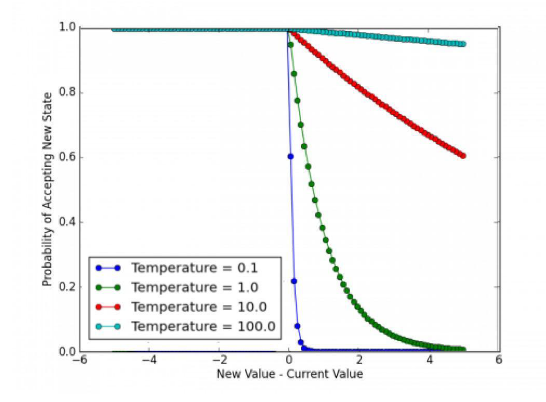
\includegraphics[width=0.6\columnwidth]{img/temp1}
\end{center}

Notice the similarity with the ILS.\\

If you're improving you always accept, if not you accept with a probability based on temperature, the higher the temperature the more the probability to accept the solution increases.\\

\newpage

\subsubsection{Asymptotic convergence to the optimum}

Due to the acceptance rule, \textbf{the current solution} $x$ \textbf{is a random variable} (depends on the random seed given): its "\textbf{state probability}" $\pi' (x)$ (associates a value of probability to each solution) \textbf{combines on all possible predecessors} $x^{(t−1)}$ 
\begin{itemize}
	\item the "state probability" $\pi' (x^{(t−1)})$ of the predecessor
	
	\item the \textbf{probability to choose the move from} $x^{(t−1)}$ to $x$, that is \textbf{uniform}
	
	\item the \textbf{probability to accept the move}, that is
	$$ \pi_T \left(x^{(t-1)}, x\right) = \begin{cases}
		1 & \text{ if } f(x) < f \left(x^{(t-1)}\right) \\
		e^{\frac{f\left(x^{(t-1)}\right) - f(x)}{T}} & \text{ if } f(x) \geq f \left(x^{(t-1)}\right) \\
	\end{cases}$$
\end{itemize}

The probability of being in a given solution $x$ in step $t$ is the combination of all the possible probabilities of the previous step, combined with the probability of choosing that specific solution from the previous step (uniform probability, it's random) and the probability of accepting said solution (stated in the formula).\\

As it \textbf{depends only on the previous step}, the solution is a \textbf{Markov chain}.\\

For fixed temperature $T$, the \textbf{transition probabilities are stationary}: it is a \textbf{homogeneous Markov chain}.\\

If the search graph for neighborhood $N$ is connected, the \textbf{probability to reach each state is} $> 0$: it is an \textbf{irreducible Markov chain}.\\

Under these assumptions (irreducible and homogeneous Markov chain), \textbf{the state probability converges to a stationary distribution independent of the starting state}. \\
For any starting state, the probability of being in a given solution after a long time tends to assume a stationary distribution, i.e., the behavior of the algorithm is not influenced by the starting solution.\\

The stationary distribution favors "good" solutions with the same law imposed by thermodynamics on physical systems at thermal equilibrium
$$ \pi_T (x) = \frac{ e^{\frac{-f(x)}{T}} }{ \sum_{x \in X} e^{\frac{-f(x)}{T}} } \text{ for each } x \in X $$

where $X$ is the feasible region and $T$ the "temperature" parameter.\\

The \textbf{distribution converges} to a \textbf{limit distribution} as $T \rightarrow 0$
$$ \pi (x) = \lim_{T \rightarrow 0} \pi_T (x) = \begin{cases}
	\frac{1}{|X^\ast|} & \text{ for } x \in X^\ast \\
	0 & \text{ for } x \in X \setminus X^\ast\\
\end{cases}$$
which corresponds to a \textbf{certain convergence to a globally optimal solution}.\\

This result however holds at the equilibrium, in infinite time.\\

In practice, \textbf{low values of} $T$ imply
\begin{itemize}
	\item a \textbf{high probability to visit a global optimum}, but also
	\item a \textbf{slow convergence} to the optimum (many exchanges are rejected)
\end{itemize}

In a finite time, the result obtained with \textbf{low} $T$ can be \textbf{far from optimal}.\\
Hence, $T$ \textbf{starts high} and is progressively updated \textbf{decreasing over time}.\\

The \textbf{starting value} $T^{[0]}$ should be
\begin{itemize}
	\item \textbf{high enough} to allow \textbf{reaching any solution quickly}
	\item \textbf{small enough} to \textbf{discourage visiting very bad solutions}
\end{itemize}

A classical tuning for $T^{[0]}$ is to
\begin{itemize}
	\item sample the first neighborhood $N (x^{(0)})$
	\item set a parameter $\beta \in (0, 1)$
	\item set $T^{[0]}$ to accept on average a fraction $\beta$ of the sampled solutions
\end{itemize}

\newpage

\subsubsection{Temperature update}
The temperature is \textbf{updated by subsequent phases} $(r = 0, \, ... \, , m)$
\begin{itemize}
	\item \textbf{each phase} applies a \textbf{constant value} $T^{[r]}$ \textbf{for} $\ell^{[r ]}$ iterations
	
	\item $T^{[r]}$ \textbf{decreases exponentially from phase to phase}
	$$ T^{[r ]} := \alpha T^{[r −1]} = \alpha^r T^{[0]} \text{ with } \alpha \in (0, 1) $$
	
	\item $\ell^{[r ]}$ \textbf{increases from phase to phase} (often linearly) \textbf{with values related to the diameter of the search graph} (therefore to the size of the instance)
\end{itemize}

Since $T$ is variable, the Markov chain $x$ is not homogeneous, but
\begin{itemize}
	\item if $T$ \textbf{decreases slowly enough}, it \textbf{converges to the global optimum}
	
	\item \textbf{good parameters} to tune the decrease \textbf{depend on the instance} (namely, on $f (\tilde{x}) - f (x^\ast)$, where $f (\tilde{x})$ is the second-best value of $f$; but the best parameter values are not known a priori)
\end{itemize}

\textbf{Adaptive SA} variants \textbf{tune the temperature} $T$ \textbf{based on the results}
\begin{itemize}
	\item \textbf{set} $T$ to a value such that a given \textbf{fraction of} $N (x)$ is \textbf{accepted}
	
	\item \textbf{increase} $T$ if the \textbf{solution has not improved for a certain time} (diversification); \textbf{otherwise decrease it} (intensification)
\end{itemize}

\newpage

\subsection{Tabu Search}
The Tabu Search (TS) has been proposed by Glover (1986).\\

It keeps the basic selection rule of steepest descent
$$ x' := \arg \min_{x \in N(x)} f (x) $$

\textbf{without the termination condition} (but this implies cycling!).\\

The TS imposes a tabu to \textbf{forbid the solutions already visited}
$$ x' := \arg \min_{x \in N(x) \setminus X_V} f(x) $$

where $X_V$ is the set of the already visited solutions.\\

\paragraph{Exchange heuristics with tabu:} An exchange heuristic that explores a neighborhood imposing a tabu on the already visited solutions requires to:
\begin{enumerate}
	\item \textbf{evaluate the feasibility} of each subset produced by the exchanges (unless guaranteed a priori)
	
	\item \textbf{evaluate the cost} of each feasible solution
	
	\item \textbf{evaluate the tabu status} of each feasible promising solution
	
\end{enumerate}
in order to \textbf{select the feasible best non-tabu solution}.\\

An elementary way to implement the evaluation of the tabu is
\begin{itemize}
	\item save the visited solutions in a suitable structure (tabu list)
	\item check each explored solution making a query on the tabu list
\end{itemize}

\newpage

\paragraph{Potential inefficiency of the tabu mechanism:} This elementary evaluation of the tabu however is \textbf{very inefficient}
\begin{itemize}
	\item the \textbf{comparison of the solutions} at step $t$ requires \textbf{time} $O (t)$ (reducible with hash tables or search trees)
	\item the \textbf{number of solutions} visited \textbf{grows indefinitely} over time
	\item the \textbf{memory occupation grows indefinitely} over time
\end{itemize}

The \textbf{Cancellation Sequence Method} and the \textbf{Reverse Elimination Method} tackle these problems, exploiting the fact that in general
\begin{itemize}
	\item the \textbf{solutions visited} form a \textbf{chain with small variations}
	\item the \textbf{solutions visited} are \textbf{rarely neighbors} of the \textbf{current one}
\end{itemize}

The idea is to \textbf{focus on variations}
\begin{itemize}
	\item \textbf{save move lists}, instead of solutions
	\item \textbf{evaluate} the \textbf{overall performed variations}, instead of the single moves
	\item \textbf{find the solutions which have undergone small overall variations} (recent ones or submitted to variations subsequently reversed)
\end{itemize}

\vfill

\paragraph{Potential ineffectiveness of the tabu mechanism:} Other subtle phenomena influence the \textbf{effectiveness of the method}.\\

\textbf{Forbidding the solutions visited} can have two different \textbf{negative effects}:
\begin{itemize}
	\item it can \textbf{disconnect the search graph}, creating impassable "iron curtains" that block the search (the prohibition should not be permanent)
	
	\item it can \textbf{slow down the exit from attraction basins}, creating a "gradual filling" effect that slows down the search (the prohibition should be extended)
\end{itemize}

The two phenomena suggest apparently opposite remedies. How to combine them? \\

\newpage

\subsubsection{Reducing potential ineffectiveness}

Some simple devices can be adopted in order to control these problems.\\

\paragraph{Attribute-based tabu:} Forbid all \textbf{solutions that share "attributes" with the visited ones}.\\

Forbidding only the visited solution slows down the search, so instead
\begin{itemize}
	\item define a \textbf{set} $A$ \textbf{of attributes} (general attributes that any solution can have)
	
	\item define \textbf{for each solution} $x \in X$ a \textbf{subset of attributes} $A_x \subseteq A$ (what attributes does each solution have)
	
	\item declare a \textbf{subset of tabu attributes} $\overline{A} \subseteq A$ (empty at first; what attributes are forbidden)
	
	\item \textbf{forbid} all the \textbf{solutions with tabu attributes}
	$$ x \text{ is tabu } \Leftrightarrow A_x \cap \overline{A} \neq \emptyset $$
	(if the solution has an attribute inside $\overline{A}$ then forbid it)
	
	\item \textbf{move from} the current solution $x$ \textbf{to} $x'$ such that $A_{x'} \cap \overline{A} = \emptyset$ (the new solution has no forbidden attributes) and add to $\overline{A}$ the attributes possessed by $x$ and not by $x'$
	$$ \overline{A} := \overline{A} \cup (A_x \setminus A{x'} ) $$
	(in this way, $x$ becomes tabu)
\end{itemize}
You don't check a list of tabu solutions, the criteria to forbid a solution is the intersection of its attributes with the set of forbidden ones.\\

This allows to
\begin{itemize}
	\item \textbf{avoid} also \textbf{solutions similar to the visited ones}
	\item \textbf{get} more quickly \textbf{far away from visited local optima}
\end{itemize}

\newpage

The \textbf{concept of "attribute"} is intentionally \textbf{generic}; the simpler ones are
\begin{itemize}
	\item \textbf{Inclusion of an element in the solution} ($A = B$ and $A_x = x$): when the move from $x$ to $x'$ expels an element $i$ from the solution, the tabu forbids the reinsertion of $i$ in the solution
	\begin{itemize}
		\item $x$ has the attribute "presence of $i$" and $x'$ hasn't got it
		\item the attribute "presence of $i$" enters $\overline{A}$
		\item every solution including $i$ becomes tabu
	\end{itemize}
	\nn
	
	\item \textbf{Exclusion of an element from the solution} ($A = B$ and $A_x = B \setminus x$): when the move from $x$ to $x'$ inserts an element $i$ into the solution, the tabu forbids the removal of $i$ from the solution
	\begin{itemize}
		\item $x$ has the attribute "absence of $i$" and $x'$ hasn't got it
		\item the attribute "absence of $i$" enters $\overline{A}$
		\item every solution devoid of $i$ becomes tabu
	\end{itemize}
	\nn
\end{itemize}

\textbf{Different attribute sets can be combined}, each with its tenure and list (e.g., after replacing $i$ with $j$, forbid both to remove $j$ and to insert $i$).\\

Other (less frequent) examples of attributes:
\begin{itemize}
	\item the \textbf{value of the objective function}: forbid solutions of a given value, previously assumed by the objective
	\item the \textbf{value of an auxiliary function}
\end{itemize}

Complex attributes can be obtained combining simple attributes
\begin{itemize}
	\item the \textbf{coexistence} in the solution \textbf{of two elements} (or their separation) 
	\item or, if a move replaces element $i$ with element $j$, the tabu can \textbf{forbid the removal of} $j$ \textbf{to include} $i$, but allow the simple removal of $j$ and the simple inclusion of $i$
\end{itemize}

\newpage

Other solutions:

\paragraph{Give a limited length $L$ (tabu tenure) to the prohibition:} The tabu mechanism creates regions hard or impossible to reach
\begin{itemize}
	\item the \textbf{tabu solutions} become \textbf{feasible again after a while}
	
	\item the \textbf{same solutions can be revisited} (but, if $\overline{A}$ is different, the \textbf{future evolution will be different}, if the evolution is the same you're stuck in a cycle)
\end{itemize}

Tuning the tabu tenure is fundamental for the effectiveness of TS\\

\paragraph{Introduce an aspiration criteria:} The tabu could forbid a global optimum similar to a visited solution, so a tabu solution \textbf{better than the best known} one is anyway \textbf{accepted} (obviously, there is no risk of looping).\\

There are looser aspiration criteria, but they are not commonly used.\\

\paragraph{If all neighbour solutions are tabu, accept the one with the oldest tabu:} The tabu could forbid all neighbour solutions. It can be interpreted as another aspiration criteria.\\
Otherwise the algorithm would just "sit still" and waste time until a tabu expires.\\

\newpage

\subsubsection{General scheme of the TS}

\begin{algorithm}
	\caption{Algorithm $TabuSearch(I , x^{(0)}, L)$}
	\begin{algorithmic}
		\STATE $x := x^{(0)}$ 
		\STATE $x^\ast := x^{(0)}$
		\STATE $\overline{A} := \emptyset$
		\WHILE{$Stop() = false$}
		\STATE $f' := + \infty$
		\FOR{each $y \in N (x)$}
		\IF{$f (y ) < f'$}
		\IF{$Tabu(y , \overline{A}) = false$ or $f(y) < f (x^\ast)$} 
		\STATE $x' := y$
		\STATE $f' := f (y )$
		\ENDIF
		\ENDIF
		\ENDFOR
		\STATE $\overline{A} := Update( \overline{A}, x', L)$
		\IF{$f (x') < f (x^\ast)$} 
		\STATE $x^\ast := x'$
		\ENDIF
		\ENDWHILE
		\RETURN $(x^\ast, f (x^\ast))$
	\end{algorithmic}
\end{algorithm}

Until the termination condition holds, for each neighbor solution finds which one is the best one; if they're not tabu or if they meet the aspiration criteria, they become the new chosen solution.\\
After every inner loop it updates the tabu list with the elements of the new solution found and the tenure of already forbidden elements (represented with $L$).\\

\newpage

\subsubsection{Efficient evaluation of the tabu status}

The \textbf{evaluation} of the tabu status must be \textbf{efficient} and avoid scanning the whole solution (as for feasibility and cost)
\begin{itemize}
	\item the \textbf{attributes are associated to moves, not to solutions}: do not check whether the solution includes $i$, but whether the move adds $i$
\end{itemize}

Let $T_i$ be the iteration when attribute $i \in A$ became tabu ($-\infty$ if $i \notin \overline{A}$).\\

To \textbf{evaluate} the tabu status in \textbf{constant time} simply \textbf{check}
$$ t \leq T_i + L $$

If the tabu is on insertions $(A = x)$, at iteration $t$
\begin{itemize}
	\item forbid the moves that add $i \in B \setminus x$ when $t \leq T_i^{in} + L^{in}$
	
	\item update $T_i^{in} := t$ for each $i$ removed $(i \in x \setminus x')$
\end{itemize}

If the tabu is on deletions $(A = B \setminus x)$, at iteration $t$
\begin{itemize}
	\item forbid the moves that delete $i \in x$ when $t \leq T_i^{out} + L^{out}$
	
	\item update $T_i^{out} := t$ for each $i$ added $(i \in x' \setminus x)$
\end{itemize}

As either $i \in x$ or $i \in B \setminus x$, \textbf{a single vector} $T$ \textbf{is enough for both checks} (an element can either be in or out).\\

More sophisticated attributes require more complex structures.\\

\newpage

\paragraph{Example:} the TSP. Consider the neighborhood $N_{\mathcal{R}_2}$ generated by 2-opt exchanges and use as attributes both the presence and the absence of arcs in the solution
\begin{itemize}
	\item At first set $T_{ij} = -\infty$ for each arc $(i, j) \in A$.\\
	
	\item At each step $t$, explore the $n(n − 1)/2$ pairs of removable arcs and the corresponding pairs of arcs which would replace them.\\
	
	\item The move $(i, j)$, which replaces $(s_i , s_{i+1})$ and $(s_j , s_{j+1})$ with $(s_i , s_j )$ and $(s_{i+1}, s_{j+1})$, is tabu at step $t$ if one of the following conditions holds:
	\begin{enumerate}
		\item $t \leq T_{s_i ,s_{i+1}} + L^{out}$
		\item $t \leq T_{s_j ,s_{j+1}} + L^{out}$
		\item $t \leq T_{s_i ,s_j} + L^{in}$
		\item $t \leq T_{s_{j+1},s_{i+1}} + L^{in}$
	\end{enumerate}
	So, at first all moves are legal. This is basically checking if all the addition and deletion moves respect the tabu conditions; check when the arcs to add were expelled and when the arcs to remove were added, and if it's long enough ago (possibly never) they are not tabu (the value $+$ tenure must be lower than $t$).\\
	If any of these conditions holds, one of the elements is tabu and the move is forbidden.\\
	
	\item For the selected move $(i^\ast, j^\ast$), update the auxiliary structures setting
	\begin{enumerate}
		\item $T_{s_{i^\ast} ,s_{i^\ast + 1}} := t$
		\item $T_{s_{j^\ast} ,s_{j^\ast + 1}} := t$
		\item $T_{s_{i^\ast} ,s_{j^\ast}} := t$
		\item $T_{s_{j^\ast + 1},s_{i^\ast + 1}} := t$
	\end{enumerate}
	Set the value of $T$ to the number of the current iteration for the affected arcs.\\
\end{itemize}

As $n$ arcs are in and $n(n − 2)$ out of the solution, it is better to set $L^{out} \ll L^{in}$. This also holds for every problem in which the solution is much smaller than the ground set (often).\\

\newpage

\paragraph{Example:} the Max-SAT. Consider the neighborhood $N_{\mathcal{F}_1}$, which includes the solutions obtained complementing the value of a variable (all $n$ solutions are feasible; one flip neighborhood).\\

Since $|x| = |B \setminus x|$ for each $x \in X$ (the number of elements in the solution are the same as the number of elements outside)
\begin{itemize}
	\item the tabu tenure for additions and deletions can be the same
	
	\item it is sufficient to forbid the change of value of a variable and the attribute is the variable
\end{itemize}

The algorithm proceeds as follows
\begin{itemize}
	\item At first, set $T_i = -\infty$ for each variable $i = 1,\, ... \, , n$.\\
	
	\item at each step $t$, explore the $n$ solutions obtained complementing each variable.\\
	
	\item the move $i$, which assigns $x_i := \overline{x}_i$ (flips the variable), is tabu at step $t$ if $t \leq T_i + L$ (it needs to be long enough since the variable has last been flipped; at first all moves are non-tabu).\\
	
	\item perform move $i^\ast$ and set $T_{i^\ast} := t$.\\
\end{itemize}

\newpage

\subsubsection{Tuning the tabu tenure}
The value of the tabu tenure $L$ is a \textbf{crucial parameter}
\begin{itemize}
	\item \textbf{too large} tenures can \textbf{conceal the global optimum} and in the worst case \textbf{block the search}
	
	\item \textbf{too small} tenures can \textbf{hold the exploration back in useless regions} and in the worst case \textbf{produce cyclic behaviors}
\end{itemize}
\nn

The \textbf{most effective value} of $L$ is in general
\begin{itemize}
	\item \textbf{related} to the \textbf{size of the instance} (big instances require more prohibition)
	
	\item \textbf{slowly growing with size} (many authors suggest $L \in O(\sqrt{|A|})$, the value of tenure grows with the square root of the value of attributes)
	
	\item but nearly \textbf{constant on medium ranges of size} (if the size doesn't change very much there's no need to change the tenure)
\end{itemize}

\textbf{Cycles can be broken} extracting $L$ at \textbf{random in a range} $[L_{min}; L_{max}]$.\\

\nn
\textbf{Adaptive mechanisms} update $L$ \textbf{based on the results} of the search within a given range $[L_{min}; L_{max}]$
\begin{itemize}
	\item \textbf{decrease} $L$ when the \textbf{current solution} $x$ \textbf{improves}: the search is probably approaching a new local optimum, and we want to favor it (intensification)
	
	\item \textbf{increase} $L$ when the \textbf{current solution} $x$ \textbf{worsens}: the search is probably leaving a known local optimum, and we want to speed up (diversification)
\end{itemize}

\newpage

\subsubsection{Variants}

Other adaptive strategies work in the long term:
\begin{itemize}
	\item \textbf{Reactive Tabu Search:}
	\begin{itemize}
		\item use efficient structures to save the solutions visited (hash table)
		\item detect cyclic behaviors (frequent repetitions)
		\item move the range $[L_{min}; L_{max}]$ upwards if the solutions repeat too often
	\end{itemize}
	\nn
	
	\item \textbf{Frequency-based Tabu Search:}
	\begin{itemize}
		\item save the frequency of each attribute in the solution in structures similar to the ones used for the tenure (e.g., $F_i$ for each $i \in B$)
		\item if an attribute appears very often
		\begin{itemize}
			\item favor the moves introducing it modifying $f$ as in the DLS
			\item forbid the moves introducing it, or discourage them by modifying $f$
		\end{itemize}
	\end{itemize}
	\nn
	
	\item \textbf{Exploring Tabu Search:} reinitialize the search from solutions of good quality which have been explored, but not used as current solution (i. e., the "second-best solutions" of some neighborhood).\\
	
	\item \textbf{Granular Tabu Search:} enlarge or reduce the neighborhood progressively.\\
\end{itemize}

% End of L19, L20 is lab, L21 from here

\newpage